\documentclass[12pt,a4paper]{article}

% ─── Page Layout ───────────────────────────────────────────────────────────────
\usepackage[a4paper, margin=0.8in, headheight=14pt]{geometry}

% ─── Fonts (XeLaTeX) ───────────────────────────────────────────────────────────
\usepackage{fontspec}
\usepackage{unicode-math}
\setmainfont{TeX Gyre Pagella}
\setmonofont[Scale=0.88]{TeX Gyre Cursor}
\setmathfont{Latin Modern Math}

% ─── Packages ──────────────────────────────────────────────────────────────────
\usepackage{xcolor}
\usepackage{colortbl}
\usepackage{titlesec}
\usepackage{enumitem}
\usepackage{tabularx}
\usepackage{booktabs}
\usepackage{array}
\usepackage{amsmath}
\usepackage{tikz}
\usetikzlibrary{shapes.geometric, arrows.meta, positioning, calc, fit, decorations.pathreplacing, patterns}
\usepackage{tcolorbox}
\tcbuselibrary{skins, breakable}
\usepackage{hyperref}
\usepackage{fancyhdr}
\usepackage{graphicx}
\usepackage{microtype}
\hyphenpenalty=10000
\exhyphenpenalty=10000
\sloppy
\usepackage{caption}
\usepackage{setspace}
\usepackage{multirow}
\usepackage{tocloft}

% ─── Q&A helper ────────────────────────────────────────────────────────────────
\newcommand{\Q}[1]{\textbf{#1}\par\noindent\ignorespaces}

% ─── Colour Palette ────────────────────────────────────────────────────────────
\definecolor{myred}{RGB}{196,30,58}
\definecolor{mydark}{RGB}{30,30,50}
\definecolor{mygreen}{RGB}{14,120,80}
\definecolor{myteal}{RGB}{0,130,140}
\definecolor{myamber}{RGB}{180,100,0}
\definecolor{mypurple}{RGB}{100,30,160}
\definecolor{mygray}{RGB}{246,247,249}
\definecolor{mgframe}{RGB}{180,185,200}
\definecolor{watermark}{RGB}{145,150,170}
\definecolor{hdrred}{RGB}{250,232,235}
\definecolor{hdrgreen}{RGB}{220,244,233}
\definecolor{hdrteal}{RGB}{220,242,244}
\definecolor{hdramber}{RGB}{253,242,215}
\definecolor{hdrpurple}{RGB}{238,228,255}
\definecolor{hdrgray}{RGB}{238,240,245}
\definecolor{rowalt}{RGB}{250,251,253}

% ─── Section Formatting ────────────────────────────────────────────────────────
\titleformat{\section}
  {\large\bfseries\color{myred}}{\thesection.}{0.5em}{}
  [\vspace{1pt}{\color{myred}\rule{\linewidth}{0.8pt}}]
\titleformat{\subsection}
  {\normalsize\bfseries\color{myteal}}{\thesubsection}{0.5em}{}
\titlespacing*{\section}{0pt}{18pt}{7pt}
\titlespacing*{\subsection}{0pt}{11pt}{4pt}

% ─── Paragraph ─────────────────────────────────────────────────────────────────
\setlength{\parindent}{0pt}
\setlength{\parskip}{4pt}

% ─── TOC Styling ───────────────────────────────────────────────────────────────
\renewcommand{\cfttoctitlefont}{\large\bfseries\color{myred}}
\renewcommand{\cftaftertoctitle}{\par\noindent{\color{myred}\rule{\linewidth}{0.8pt}}}
\setlength{\cftbeforetoctitleskip}{0pt}
\setlength{\cftaftertoctitleskip}{6pt}
\renewcommand{\cftsecfont}{\normalsize\bfseries\color{mydark}}
\renewcommand{\cftsecpagefont}{\normalsize\bfseries\color{mydark}}
\renewcommand{\cftsecleader}{\cftdotfill{\cftdotsep}}
\setlength{\cftbeforesecskip}{7pt}
\renewcommand{\cftsubsecfont}{\small\color{mydark}}
\renewcommand{\cftsubsecpagefont}{\small\color{mydark}}
\setlength{\cftbeforesubsecskip}{3pt}
\setlength{\cftsubsecindent}{1.4em}

% ─── Table helpers ─────────────────────────────────────────────────────────────
\renewcommand{\arraystretch}{1.45}
\setlength{\tabcolsep}{6pt}
\arrayrulecolor{mydark}
\newcolumntype{B}[1]{>{\small\bfseries\raggedright\arraybackslash}m{#1}}
\newcolumntype{Y}{>{\small\raggedright\arraybackslash}X}
\renewcommand{\tabularxcolumn}[1]{m{#1}}

% ─── Header / Footer ───────────────────────────────────────────────────────────
\pagestyle{fancy}
\fancyhf{}
\fancyhead[L]{\small\color{myred}\textbf{ES-CS301}\;\color{mydark}--- Data Structure \& Algorithms}
\fancyhead[R]{\small\color{myteal}\textbf{Module 2 Notes}}
\fancyfoot[C]{\small\color{mydark}\thepage}
\fancyfoot[R]{\small\color{watermark}\textit{\copyright\ Biraj}}
\renewcommand{\headrulewidth}{0.5pt}
\renewcommand{\footrulewidth}{0.3pt}

% ─── Hyperref ──────────────────────────────────────────────────────────────────
\hypersetup{
  colorlinks=true, linkcolor=myteal, urlcolor=myteal,
  pdfauthor={Biraj Sarkar (CGEC)},
  pdftitle={ES-CS301 --- Module 2 Notes: Stacks and Queues: ADTs, Operations and Applications}
}

% ─── tcolorbox styles ──────────────────────────────────────────────────────────
\tcbset{
  tikzbox/.style={
    colback=mygray, colframe=mgframe, boxrule=0.6pt, arc=4pt,
    left=8pt, right=8pt, top=6pt, bottom=6pt,
    colbacktitle=mgframe, coltitle=mydark,
    fonttitle=\small\bfseries
  },
  defbox/.style={
    colback=hdrgreen, colframe=mygreen, boxrule=0.8pt, arc=4pt,
    left=9pt, right=9pt, top=6pt, bottom=6pt,
    colbacktitle=mygreen, coltitle=white,
    fonttitle=\small\bfseries
  },
  formulabox/.style={
    colback=hdrteal, colframe=myteal, boxrule=0.8pt, arc=4pt,
    left=9pt, right=9pt, top=7pt, bottom=7pt,
    colbacktitle=myteal, coltitle=white,
    fonttitle=\small\bfseries
  },
  examplebox/.style={
    colback=hdramber, colframe=myamber, boxrule=0.8pt, arc=4pt,
    left=9pt, right=9pt, top=6pt, bottom=6pt,
    colbacktitle=myamber, coltitle=white,
    fonttitle=\small\bfseries
  },
  masonbox/.style={
    colback=hdrpurple, colframe=mypurple, boxrule=0.8pt, arc=4pt,
    left=9pt, right=9pt, top=6pt, bottom=6pt,
    colbacktitle=mypurple, coltitle=white,
    fonttitle=\small\bfseries
  },
  exambox/.style={
    colback=hdrpurple, colframe=mypurple, boxrule=1pt, arc=5pt,
    left=10pt, right=10pt, top=8pt, bottom=8pt,
    colbacktitle=mypurple, coltitle=white,
    fonttitle=\bfseries,
    breakable, title after break={\textbf{Frequently Asked / Viva Questions (contd.)}}
  }
}

\tcbset{breakable}
\tcbset{after={\color{black}}}

% ─── TikZ styles ───────────────────────────────────────────────────────────────
\tikzset{
  stackslot/.style={rectangle, draw=myteal, fill=hdrteal, minimum width=2.4cm, minimum height=0.7cm, align=center, font=\small\bfseries},
  queueslot/.style={rectangle, draw=mygreen, fill=hdrgreen, minimum width=1.1cm, minimum height=1.1cm, align=center, font=\small\bfseries},
  arrow/.style={-Stealth, thick, color=mydark},
  redarrow/.style={-Stealth, thick, color=myred},
  line/.style={thick, color=mydark}
}

\begin{document}

% ─── Title Page ───────────────────────────────────────────────────────────────
\begin{center}
  {\LARGE\bfseries\color{myred} ES-CS301 --- Data Structure \& Algorithms}\\[5pt]
  {\normalsize\color{mydark} Semester III \quad$\bullet$\quad 3L:0T:4P \quad$\bullet$\quad 3 Credits}\\[3pt]
  {\normalsize\color{myteal}\textbf{Module 2 Exam Notes: Stacks and Queues: Principles, Operations and Applications}}\\[3pt]
  {\small\color{mydark} CGEC \;$|$\; B.Tech ECE (2023--27) \;$|$\; \textit{Biraj Sarkar}}
\end{center}
\vspace{2pt}
\noindent{\color{myred}\rule{\linewidth}{1.5pt}}
\vspace{2pt}

\hypersetup{linkcolor=mydark}
\tableofcontents
\hypersetup{linkcolor=myteal}
\newpage

% ───────────────────────────────────────────────────────────────────────────────
\section{Abstract Data Type Stack and Fundamental Operations}
% ───────────────────────────────────────────────────────────────────────────────

\begin{tcolorbox}[defbox, title={\textbf{Definition: Stack Abstract Data Type (ADT)}}]
A \textbf{Stack} is a linear, restricted-access data structure adhering strictly to the \textbf{Last-In, First-Out (LIFO)} or \textbf{First-In, Last-Out (FILO)} operating discipline. All insertions (\texttt{push}) and deletions (\texttt{pop}) are constrained to take place at a single end termed the \textbf{Top of Stack (TOS)}.
\par\vspace{4pt}
Formally, a Stack $S$ over an element domain $E$ is defined by:
\begin{itemize}[leftmargin=*, nosep]
  \item State: An ordered sequence $S = \langle e_0, e_1, \dots, e_k \rangle$ where $e_k$ is the Top element.
  \item Auxiliary Pointer: An integer index $\text{top} \in [-1, \text{MAX}-1]$ indicating the index of the most recently inserted item.
\end{itemize}
\end{tcolorbox}

\subsection{Array Implementation of Stack}
In an array-based static implementation, elements reside in contiguous storage $S[0 \dots \text{MAX}-1]$.
\begin{itemize}[leftmargin=*, itemsep=3pt]
  \item \textbf{Initial Condition:} $\text{top} = -1$ (stack is strictly empty).
  \item \textbf{Stack Overflow Condition:} Attempting to insert an element when the physical capacity is exhausted:
  \begin{equation}
    \text{Overflow} \iff \text{top} == \text{MAX} - 1
  \end{equation}
  \item \textbf{Stack Underflow Condition:} Attempting to retrieve or delete an element from an empty stack:
  \begin{equation}
    \text{Underflow} \iff \text{top} == -1
  \end{equation}
\end{itemize}

\begin{tcolorbox}[formulabox, title={\textbf{Core Stack Primitive Algorithms and Complexity Bounds}}]
\textbf{1. Algorithm Push($S, \text{top}, x$):}
\begin{verbatim}
if (top == MAX - 1)
    report "Stack Overflow" and exit error;
top = top + 1;
S[top] = x;
\end{verbatim}
Time Complexity: $\mathbf{\mathcal{O}(1)}$ \quad Space Complexity: $\mathbf{\mathcal{O}(1)}$

\par\vspace{3pt}\noindent
\textbf{2. Algorithm Pop($S, \text{top}$):}
\begin{verbatim}
if (top == -1)
    report "Stack Underflow" and exit error;
item = S[top];
top = top - 1;
return item;
\end{verbatim}
Time Complexity: $\mathbf{\mathcal{O}(1)}$ \quad Space Complexity: $\mathbf{\mathcal{O}(1)}$

\par\vspace{3pt}\noindent
\textbf{3. Algorithm Peek($S, \text{top}$):}
\begin{verbatim}
if (top == -1)
    report "Stack Empty" and exit error;
return S[top]; // Non-destructive inspection
\end{verbatim}
Time Complexity: $\mathbf{\mathcal{O}(1)}$ \quad Space Complexity: $\mathbf{\mathcal{O}(1)}$
\end{tcolorbox}

\begin{tcolorbox}[tikzbox, title={\textbf{LIFO Mechanism and State Transitions in Stack Operations}}]
\centering
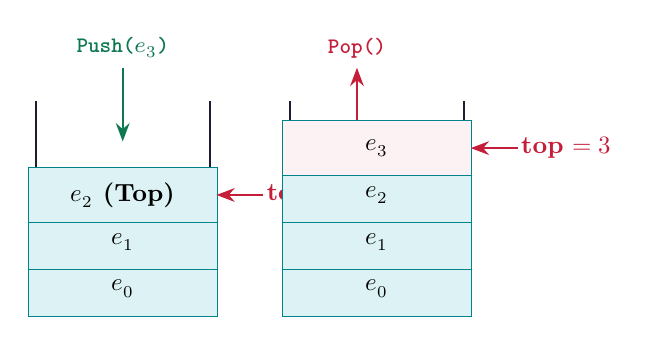
\begin{tikzpicture}[scale=0.85, every node/.style={font=\small}]
  % Stack slots
  \draw[thick, mydark] (0,3.2) -- (0,0) -- (2.6,0) -- (2.6,3.2);
  \node[stackslot] at (1.3,0.4) {$e_0$};
  \node[stackslot] at (1.3,1.1) {$e_1$};
  \node[stackslot] at (1.3,1.8) {$e_2$ (Top)};

  \draw[redarrow] (3.4,1.8) -- (2.7,1.8) node[midway, right=6pt] {\textbf{top} $= 2$};

  % Push Action
  \draw[arrow, mygreen] (1.3,3.7) -- (1.3,2.6);
  \node[above, font=\footnotesize\bfseries, color=mygreen] at (1.3,3.7) {\texttt{Push($e_3$)}};

  % Pop Action
  \draw[arrow, myred] (4.8,2.6) -- (4.8,3.7);
  \node[above, font=\footnotesize\bfseries, color=myred] at (4.8,3.7) {\texttt{Pop()}};
  \draw[thick, mydark] (3.8,3.2) -- (3.8,0) -- (6.4,0) -- (6.4,3.2);
  \node[stackslot] at (5.1,0.4) {$e_0$};
  \node[stackslot] at (5.1,1.1) {$e_1$};
  \node[stackslot] at (5.1,1.8) {$e_2$};
  \node[stackslot, fill=hdrred!60] at (5.1,2.5) {$e_3$};
  \draw[redarrow] (7.2,2.5) -- (6.5,2.5) node[midway, right=6pt] {\textbf{top} $= 3$};
\end{tikzpicture}
\end{tcolorbox}

% ───────────────────────────────────────────────────────────────────────────────
\section{Applications of Stacks}
% ───────────────────────────────────────────────────────────────────────────────

\subsection{Arithmetic Expression Formats and Operator Precedence}
Mathematical expressions are represented in three distinct syntactic notations:
\begin{enumerate}[leftmargin=*, itemsep=3pt]
  \item \textbf{Infix Notation:} Binary operators are placed between operands: $\langle \text{Operand} \rangle \; \mathbf{Op} \; \langle \text{Operand} \rangle$ (e.g., $(A + B) * C$). Requires explicit parentheses and precedence parsing rules.
  \item \textbf{Postfix Notation (Reverse Polish Notation --- RPN):} Operators appear immediately following their operands: $\langle \text{Operand} \rangle \; \langle \text{Operand} \rangle \; \mathbf{Op}$ (e.g., $A B + C *$). Evaluated linearly without parentheses or backtrack searching.
  \item \textbf{Prefix Notation (Polish Notation):} Operators precede operands: $\mathbf{Op} \; \langle \text{Operand} \rangle \; \langle \text{Operand} \rangle$ (e.g., $* + A B C$).
\end{enumerate}

\par\vspace{6pt}\noindent
\begingroup
\setlength{\tabcolsep}{5pt}
\setlength{\extrarowheight}{3pt}
\renewcommand{\arraystretch}{1.3}
\begin{tabularx}{\linewidth}{|B{3.2cm}|B{3.5cm}|B{2.8cm}|Y|}
\hline
\textbf{Operator} & \textbf{Operation Description} & \textbf{Associativity} & \textbf{Precedence Rank} \\
\hline
\texttt{\^{}} or \texttt{\$} & Exponentiation & Right-to-Left ($\text{R} \to \text{L}$) & Highest (Rank 3) \\
\hline
\texttt{*}, \texttt{/}, \texttt{\%} & Multiplication, Division, Modulo & Left-to-Right ($\text{L} \to \text{R}$) & Intermediate (Rank 2) \\
\hline
\texttt{+}, \texttt{-} & Addition, Subtraction & Left-to-Right ($\text{L} \to \text{R}$) & Lowest (Rank 1) \\
\hline
\texttt{(} & Left Parenthesis & Left-to-Right & Rank 0 (Inside Stack) \\
\hline
\end{tabularx}
\endgroup

\subsection{Infix to Postfix Conversion Algorithm}
\begin{tcolorbox}[defbox, title={\textbf{Shunting-Yard Infix to Postfix Algorithm}}]
\begin{enumerate}[leftmargin=*, nosep]
  \item Initialize an empty operator stack $S$ and an empty postfix output string $P$.
  \item Scan the infix expression string $I$ from left to right, character by character:
  \begin{itemize}[leftmargin=*, nosep]
    \item \textbf{If Operand:} Append directly to postfix string $P$.
    \item \textbf{If Left Parenthesis \texttt{'('}:} Push onto stack $S$.
    \item \textbf{If Right Parenthesis \texttt{')'}:} Pop from $S$ and append to $P$ repeatedly until \texttt{'('} is popped. Discard both parentheses.
    \item \textbf{If Operator $op$:} While stack is non-empty, and $\text{Prec}(\text{top}) > \text{Prec}(op)$ (or $\text{Prec}(\text{top}) == \text{Prec}(op)$ with Left-Associativity), pop $S$ and append to $P$. Then push $op$ onto $S$.
  \end{itemize}
  \item After end of input string, pop all remaining operators from $S$ and append to $P$.
\end{enumerate}
\end{tcolorbox}

\begin{tcolorbox}[examplebox, title={\textbf{Step-by-Step Trace: Infix to Postfix Conversion}}]
Convert: $I = A + B * (C \wedge D - E) \wedge (F + G * H) - I$
\par\vspace{4pt}
\begingroup
\setlength{\tabcolsep}{4.5pt}
\setlength{\extrarowheight}{1.5pt}
\renewcommand{\arraystretch}{1.15}
\begin{tabularx}{\linewidth}{|B{1.6cm}|B{2.8cm}|Y|B{3.2cm}|}
\hline
\textbf{Token} & \textbf{Operator Stack} & \textbf{Postfix Output $P$} & \textbf{Action} \\
\hline
$A$ & $\emptyset$ & $A$ & Append operand \\
$+$ & $+$ & $A$ & Push operator \\
$B$ & $+$ & $A B$ & Append operand \\
$*$ & $+ \; *$ & $A B$ & Push (higher precedence) \\
$($ & $+ \; * \; ($ & $A B$ & Push parenthesis \\
$C$ & $+ \; * \; ($ & $A B C$ & Append operand \\
$\wedge$ & $+ \; * \; ( \; \wedge$ & $A B C$ & Push exponent \\
$D$ & $+ \; * \; ( \; \wedge$ & $A B C D$ & Append operand \\
$-$ & $+ \; * \; ( \; -$ & $A B C D \wedge$ & Pop $\wedge$, push $-$ \\
$E$ & $+ \; * \; ( \; -$ & $A B C D \wedge E$ & Append operand \\
$)$ & $+ \; *$ & $A B C D \wedge E -$ & Pop until $($, discard \\
$\wedge$ & $+ \; * \; \wedge$ & $A B C D \wedge E -$ & Push (higher precedence) \\
$($ & $+ \; * \; \wedge \; ($ & $A B C D \wedge E -$ & Push parenthesis \\
$F$ & $+ \; * \; \wedge \; ($ & $A B C D \wedge E - F$ & Append operand \\
$+$ & $+ \; * \; \wedge \; ( \; +$ & $A B C D \wedge E - F$ & Push operator \\
$G$ & $+ \; * \; \wedge \; ( \; +$ & $A B C D \wedge E - F G$ & Append operand \\
$*$ & $+ \; * \; \wedge \; ( \; + \; *$ & $A B C D \wedge E - F G$ & Push (higher precedence) \\
$H$ & $+ \; * \; \wedge \; ( \; + \; *$ & $A B C D \wedge E - F G H$ & Append operand \\
$)$ & $+ \; * \; \wedge$ & $A B C D \wedge E - F G H * +$ & Pop until $($, discard \\
$-$ & $-$ & $A B C D \wedge E - F G H * + \wedge * +$ & Pop $\wedge, *, +$, push $-$ \\
$I$ & $-$ & $A B C D \wedge E - F G H * + \wedge * + I$ & Append operand \\
\textbf{End} & $\emptyset$ & $\mathbf{A B C D \wedge E - F G H * + \wedge * + I -}$ & Pop all remaining \\
\hline
\end{tabularx}
\endgroup
\end{tcolorbox}

\subsection{Evaluation of Postfix Expressions}
\begin{tcolorbox}[formulabox, title={\textbf{Postfix Expression Evaluation Algorithm}}]
Scan postfix string $P$ from left to right:
\begin{enumerate}[leftmargin=*, nosep]
  \item If current symbol is an operand, push its numerical value onto operand stack $S$.
  \item If symbol is an operator $\odot$:
  \begin{itemize}[leftmargin=*, nosep]
    \item $\text{op}_2 = \text{Pop}(S)$ \quad \textit{(Second operand popped first!)}
    \item $\text{op}_1 = \text{Pop}(S)$ \quad \textit{(First operand popped second!)}
    \item Compute $\text{result} = \text{op}_1 \odot \text{op}_2$.
    \item $\text{Push}(S, \text{result})$.
  \end{itemize}
  \item When string ends, the final evaluated result resides at $\text{Pop}(S)$.
\end{enumerate}
Time Complexity: $\mathbf{\mathcal{O}(n)}$ \quad Auxiliary Space: $\mathbf{\mathcal{O}(n)}$
\end{tcolorbox}

\begin{tcolorbox}[examplebox, title={\textbf{Evaluation Trace: Numerical Postfix String}}]
Evaluate: $P = 6 \; 2 \; 3 \; + \; * \; 12 \; 4 \; / \; -$
\begin{itemize}[leftmargin=*, itemsep=2pt]
  \item Scan \texttt{6}, \texttt{2}, \texttt{3}: Push to stack $\implies S = [6, 2, 3]$.
  \item Encounter \texttt{+}: Pop $\text{op}_2 = 3$, $\text{op}_1 = 2$. Compute $2 + 3 = 5$. Push $5 \implies S = [6, 5]$.
  \item Encounter \texttt{*}: Pop $\text{op}_2 = 5$, $\text{op}_1 = 6$. Compute $6 * 5 = 30$. Push $30 \implies S = [30]$.
  \item Scan \texttt{12}, \texttt{4}: Push to stack $\implies S = [30, 12, 4]$.
  \item Encounter \texttt{/}: Pop $\text{op}_2 = 4$, $\text{op}_1 = 12$. Compute $12 / 4 = 3$. Push $3 \implies S = [30, 3]$.
  \item Encounter \texttt{-}: Pop $\text{op}_2 = 3$, $\text{op}_1 = 30$. Compute $30 - 3 = 27$. Push $27 \implies S = [27]$.
  \item End of expression: Final Result = $\mathbf{27}$.
\end{itemize}
\end{tcolorbox}

\subsection{Infix to Prefix Conversion and Prefix Evaluation}
\begin{tcolorbox}[defbox, title={\textbf{Infix to Prefix Conversion Algorithm (Reversal Method)}}]
To convert an infix expression $I$ to prefix notation $Pre$:
\begin{enumerate}[leftmargin=*, nosep]
  \item Reverse the infix string $I$.
  \item In the reversed string, replace every \texttt{'('} with \texttt{')'} and every \texttt{')'} with \texttt{'('}.
  \item Compute the postfix expression of this transformed string using the Shunting-Yard algorithm (with operator precedence rules: if precedence of scanned operator equals TOS, operators with right-associativity pop TOS, left-associative operators are pushed).
  \item Reverse the resulting postfix string. The final string is the valid \textbf{Prefix expression}.
\end{enumerate}
Time Complexity: $\mathbf{\mathcal{O}(n)}$ \quad Auxiliary Space: $\mathbf{\mathcal{O}(n)}$
\end{tcolorbox}

\begin{tcolorbox}[examplebox, title={\textbf{Example: Infix to Prefix Conversion}}]
Convert: $I = (A + B) * C - (D - E) * (F + G)$
\begin{enumerate}[leftmargin=*, nosep]
  \item Reverse $I$: $(G + F) * (E - D) - C * (B + A)$
  \item Swap brackets: $(G + F) * (E - D) - C * (B + A)$
  \item Postfix of transformed string: $G F + E D - * C B A + * -$
  \item Reverse result: $\mathbf{- * + A B C * - D E + F G}$ (or $- * + A B C * - D E + F G$)
\end{enumerate}
\end{tcolorbox}

\begin{tcolorbox}[formulabox, title={\textbf{Prefix Expression Evaluation Algorithm}}]
Scan the prefix expression $Pre$ from \textbf{Right to Left}:
\begin{enumerate}[leftmargin=*, nosep]
  \item If current symbol is an operand, push its value onto operand stack $S$.
  \item If symbol is an operator $\odot$:
  \begin{itemize}[leftmargin=*, nosep]
    \item $\text{op}_1 = \text{Pop}(S)$ \quad \textit{(First operand popped first!)}
    \item $\text{op}_2 = \text{Pop}(S)$ \quad \textit{(Second operand popped second!)}
    \item Compute $\text{result} = \text{op}_1 \odot \text{op}_2$.
    \item $\text{Push}(S, \text{result})$.
  \end{itemize}
  \item When scan completes, $\text{Pop}(S)$ contains the final evaluated scalar value.
\end{enumerate}
\end{tcolorbox}

\subsection{Balanced Delimiter Checking and Call Stack Simulation}
\begin{tcolorbox}[defbox, title={\textbf{Algorithm: Delimiter Matching (Parentheses Balancing)}}]
\textbf{Algorithm CheckBalanced($expr$):}
\begin{enumerate}[leftmargin=*, nosep]
  \item Initialize an empty character stack $S$.
  \item For each character $ch$ in string $expr$:
  \begin{itemize}[leftmargin=*, nosep]
    \item If $ch \in \{ \texttt{'('}, \texttt{'['}, \texttt{'\{'} \}$, execute $\text{Push}(S, ch)$.
    \item If $ch \in \{ \texttt{')'}, \texttt{']'}, \texttt{'\}'} \}$:
    \begin{itemize}[leftmargin=*, nosep]
      \item If $\text{IsEmpty}(S)$, return \textbf{False} (Underflow: unmatched closing bracket).
      \item $topChar = \text{Pop}(S)$.
      \item If $(topChar, ch)$ is not a matching pair \texttt{()}, \texttt{[]}, or \texttt{\{\}}, return \textbf{False}.
    \end{itemize}
  \end{itemize}
  \item Return $\text{IsEmpty}(S)$ (True if all opened brackets were closed; False otherwise).
\end{enumerate}
Time Complexity: $\mathbf{\mathcal{O}(n)}$ \quad Space Complexity: $\mathbf{\mathcal{O}(n)}$
\end{tcolorbox}

\begin{tcolorbox}[examplebox, title={\textbf{Function Call Stack and Recursion Architecture}}]
When a recursive function (such as $n!$ or Fibonacci) executes, the operating system instantiates an \textbf{Activation Record (Stack Frame)} on the thread's call stack for each recursive call:
\begin{itemize}[leftmargin=*, nosep]
  \item Contents of a Frame: Return Address, Function Parameters, Local Variables, Saved Base Pointer (\texttt{EBP/RBP}).
  \item Growth: As calls nest deeper, frames stack vertically. Winding phase consumes $\mathcal{O}(n)$ stack space.
  \item Unwinding: Upon reaching base case, frames pop in LIFO sequence, returning values to caller.
\end{itemize}
\end{tcolorbox}

% ───────────────────────────────────────────────────────────────────────────────
\section{Abstract Data Type Queue and Linear Queue}
% ───────────────────────────────────────────────────────────────────────────────

\begin{tcolorbox}[defbox, title={\textbf{Definition: Queue Abstract Data Type (ADT)}}]
A \textbf{Queue} is a linear, homogeneous data structure governed by the \textbf{First-In, First-Out (FIFO)} operating principle. Insertions are restricted to the \textbf{Rear} terminal, while deletions occur exclusively at the \textbf{Front} terminal.
\par\vspace{4pt}
Pointers in an array of size $\text{MAX}$:
\begin{itemize}[leftmargin=*, nosep]
  \item $\text{front}$: Points to the position of the first valid data element (or one position prior in alternate textbook conventions).
  \item $\text{rear}$: Points to the index of the latest inserted data item.
\end{itemize}
\end{tcolorbox}

\subsection{Array Implementation of Linear Queue}
Let array storage be $Q[0 \dots \text{MAX}-1]$ with standard $0$-based indices:
\begin{itemize}[leftmargin=*, itemsep=2pt]
  \item \textbf{Initial Empty State:} $\text{front} = -1, \; \text{rear} = -1$.
  \item \textbf{Queue Underflow Condition:} $\text{front} == -1$ (or $\text{front} > \text{rear}$).
  \item \textbf{Queue Overflow Condition:} $\text{rear} == \text{MAX} - 1$.
\end{itemize}

\begin{tcolorbox}[formulabox, title={\textbf{Linear Queue Algorithms and the False Overflow Anomaly}}]
\textbf{1. Algorithm Enqueue($Q, x$):}
\begin{verbatim}
if (rear == MAX - 1)
    report "Queue Overflow" and exit error;
if (front == -1) front = 0; // First element insertion
rear = rear + 1;
Q[rear] = x;
\end{verbatim}

\textbf{2. Algorithm Dequeue($Q$):}
\begin{verbatim}
if (front == -1 || front > rear)
    report "Queue Underflow" and exit error;
item = Q[front];
front = front + 1;
if (front > rear) // Reset queue when emptied
    front = -1, rear = -1;
return item;
\end{verbatim}
\par\vspace{2pt}\noindent
\textbf{The False Overflow Problem (Memory Drift):} In a simple linear queue, after several enqueue and dequeue cycles, $\text{rear}$ reaches $\text{MAX}-1$ while $\text{front}$ has advanced forward (e.g., $\text{front} = 4, \text{rear} = \text{MAX}-1$). Even though indices $0 \dots 3$ are physically empty, the condition $\text{rear} == \text{MAX}-1$ reports overflow and rejects new insertions!
\end{tcolorbox}

% ───────────────────────────────────────────────────────────────────────────────
\section{Advanced Queue Architectures}
% ───────────────────────────────────────────────────────────────────────────────

\subsection{Circular Queue}
A \textbf{Circular Queue} overcomes false overflow by logically connecting index $\text{MAX}-1$ back to index $0$ via \textbf{modulo arithmetic}:
\begin{equation}
  \text{next}(\text{index}) = (\text{index} + 1) \bmod \text{MAX}
\end{equation}

\begin{tcolorbox}[defbox, title={\textbf{Circular Queue Boundary States and Algorithms}}]
Let $Q[0 \dots \text{MAX}-1]$:
\begin{itemize}[leftmargin=*, itemsep=3pt]
  \item \textbf{Initial Empty State:} $\text{front} = -1, \; \text{rear} = -1$.
  \item \textbf{Circular Queue Full Condition:}
  \begin{equation}
    (\text{rear} + 1) \bmod \text{MAX} == \text{front}
  \end{equation}
  \item \textbf{Circular Queue Empty Condition:}
  \begin{equation}
    \text{front} == -1
  \end{equation}
\end{itemize}
\par\vspace{2pt}\noindent
\textbf{Algorithm CircularEnqueue($Q, x$):}
\begin{verbatim}
if ((rear + 1) % MAX == front)
    report "Circular Queue Overflow" and exit;
if (front == -1) // First element
    front = 0, rear = 0;
else
    rear = (rear + 1) % MAX;
Q[rear] = x;
\end{verbatim}

\textbf{Algorithm CircularDequeue($Q$):}
\begin{verbatim}
if (front == -1)
    report "Circular Queue Underflow" and exit;
item = Q[front];
if (front == rear) // Only one element was present
    front = -1, rear = -1;
else
    front = (front + 1) % MAX;
return item;
\end{verbatim}
\end{tcolorbox}

\begin{tcolorbox}[tikzbox, title={\textbf{Ring Representation of Circular Queue ($MAX=8$)}}]
\centering
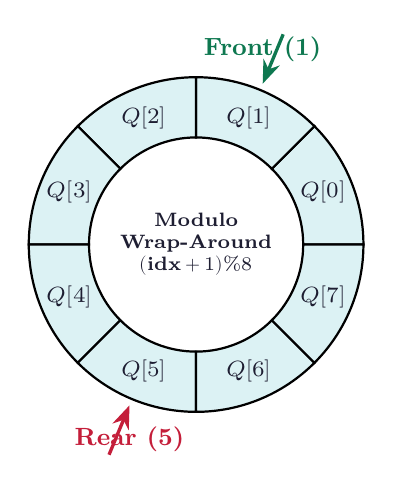
\begin{tikzpicture}[scale=0.85]
  % Draw circular ring segments
  \foreach \i in {0,1,...,7} {
    \draw[thick, fill=hdrteal] (\i*45:1.6cm) arc (\i*45:(\i+1)*45:1.6cm) -- 
          ({(\i+1)*45}:2.5cm) arc ({(\i+1)*45}:\i*45:2.5cm) -- cycle;
    \node[font=\footnotesize\bfseries, color=mydark] at (\i*45+22.5:2.05cm) {$Q[\i]$};
  }
  % Highlight front and rear
  \draw[-Stealth, very thick, color=mygreen] (67.5:3.4cm) -- (67.5:2.6cm) node[above=4pt, font=\small\bfseries] {Front (1)};
  \draw[-Stealth, very thick, color=myred] (247.5:3.4cm) -- (247.5:2.6cm) node[below=4pt, font=\small\bfseries] {Rear (5)};
  \node[font=\scriptsize\bfseries, color=mydark, align=center] at (0,0) {Modulo\\Wrap-Around\\$(\text{idx}+1)\%8$};
\end{tikzpicture}
\end{tcolorbox}

\subsection{Priority Queue}
A \textbf{Priority Queue} is an ADT where each element has an associated priority key. Elements are processed according to priority rather than arrival time:
\begin{itemize}[leftmargin=*, itemsep=3pt]
  \item \textbf{Ascending Priority Queue:} Item with the lowest numerical priority value is extracted first.
  \item \textbf{Descending Priority Queue:} Item with the highest numerical priority value is extracted first.
\end{itemize}

\par\vspace{6pt}\noindent
\begingroup
\setlength{\tabcolsep}{4.5pt}
\setlength{\extrarowheight}{3pt}
\renewcommand{\arraystretch}{1.3}
\begin{tabularx}{\linewidth}{|B{3.2cm}|B{3.0cm}|B{3.0cm}|Y|}
\hline
\textbf{Implementation} & \textbf{Enqueue Time} & \textbf{Dequeue Time} & \textbf{Trade-off Remarks} \\
\hline
Unordered Array & $\mathcal{O}(1)$ & $\mathcal{O}(n)$ & Linear search required to find extreme priority. \\
\hline
Ordered Array & $\mathcal{O}(n)$ & $\mathcal{O}(1)$ & Sorted insertion requires element shifts. \\
\hline
Unordered Linked List & $\mathcal{O}(1)$ & $\mathcal{O}(n)$ & Deletion requires traversing entire list. \\
\hline
Ordered Linked List & $\mathcal{O}(n)$ & $\mathcal{O}(1)$ & Dequeue is $\mathcal{O}(1)$ removal at head. \\
\hline
\textbf{Binary Heap} & $\mathbf{\mathcal{O}(\log n)}$ & $\mathbf{\mathcal{O}(\log n)}$ & \textbf{Optimal engineering balance} (standard in C++/Java). \\
\hline
\end{tabularx}
\endgroup

\subsection{Double-Ended Queue (DEQUE)}
A \textbf{DEQUE} (Double-Ended Queue) permits insertion and deletion at both the front and rear ends:
\begin{enumerate}[leftmargin=*, itemsep=3pt]
  \item \textbf{Input-Restricted DEQUE:} Insertion is allowed at only one end (e.g., rear), while deletion is allowed at both ends (front and rear).
  \item \textbf{Output-Restricted DEQUE:} Deletion is allowed at only one end (e.g., front), while insertion is allowed at both ends (front and rear).
\end{enumerate}

\newpage
% ===============================================================================
% MANDATORY QUICK REVISION PAGE
% ===============================================================================
\begin{center}
  {\large\bfseries\color{myred} Quick Revision --- Module 2}\\[3pt]
  {\small\color{mydark} Stacks and Queues: ADTs, Operations and Applications $|$ ES-CS301}
\end{center}
\noindent{\color{myred}\rule{\linewidth}{1.2pt}}
\vspace{4pt}

\begin{tcolorbox}[formulabox, title={\textbf{Key Formulas and Boundary Conditions at a Glance}}]
\renewcommand{\arraystretch}{1.35}
\begin{tabularx}{\linewidth}{B{5.0cm} X}
Stack Overflow Condition & $\text{top} == \text{MAX} - 1$ \\[3pt]
Stack Underflow Condition & $\text{top} == -1$ \\[3pt]
Linear Queue Empty & $\text{front} == -1 \quad \text{or} \quad \text{front} > \text{rear}$ \\[3pt]
Linear Queue Overflow & $\text{rear} == \text{MAX} - 1 \quad \text{(Susceptible to False Overflow)}$ \\[3pt]
Circular Queue Next Pointer & $\text{next} = (\text{index} + 1) \bmod \text{MAX}$ \\[3pt]
Circular Queue Full & $(\text{rear} + 1) \bmod \text{MAX} == \text{front}$ \\[3pt]
Circular Queue Empty & $\text{front} == -1$ \\[3pt]
Circular Queue Element Count & $\text{Count} = (\text{rear} - \text{front} + \text{MAX}) \bmod \text{MAX} + 1 \quad (\text{if non-empty})$ \\[3pt]
Stack Operation Complexities & $\text{Push: } \mathcal{O}(1), \quad \text{Pop: } \mathcal{O}(1), \quad \text{Peek: } \mathcal{O}(1)$ \\[3pt]
Binary Heap Priority Queue & $\text{Insert: } \mathcal{O}(\log n), \quad \text{Extract-Min/Max: } \mathcal{O}(\log n)$ \\[3pt]
\end{tabularx}
\end{tcolorbox}

\begin{tcolorbox}[defbox, title={\textbf{One-Line Definitions}}]
\begin{itemize}[leftmargin=*, itemsep=2pt, topsep=0pt]
  \item \textbf{Stack:} A linear list where insertions and deletions occur strictly at one end (LIFO discipline).
  \item \textbf{Queue:} A linear list where insertions occur at the rear and deletions at the front (FIFO discipline).
  \item \textbf{Top of Stack (TOS):} An integer pointer referencing the most recently pushed element.
  \item \textbf{False Overflow:} Rejection of enqueue requests in a linear queue when rear is at $\text{MAX}-1$ despite empty slots at the front.
  \item \textbf{Circular Queue:} A queue where the end of the array wraps around to the beginning using modulo arithmetic.
  \item \textbf{Priority Queue:} A queue where elements are retrieved based on an assigned priority key rather than FIFO order.
  \item \textbf{DEQUE:} A generalized queue permitting insertion and deletion operations at both extremities.
  \item \textbf{Infix Notation:} Arithmetic notation placing operators between operands (requires parentheses).
  \item \textbf{Postfix Notation (RPN):} Arithmetic notation placing operators after operands (parenthesis-free).
  \item \textbf{Prefix Notation:} Arithmetic notation placing operators before operands (Polish notation).
  \item \textbf{Activation Record:} A memory block pushed onto the call stack containing parameters, local variables, and return addresses.
  \item \textbf{Balanced Delimiters:} A string of grouping symbols where each opening token matches its corresponding closing token in proper nested order.
\end{itemize}
\end{tcolorbox}

\begin{tcolorbox}[exambox, title={\textbf{Frequently Asked / Viva Questions}}]
\begin{enumerate}[topsep=0pt, label=\textbf{Q\arabic*.}, itemsep=5pt]
  \item \Q{What is the primary difference between LIFO and FIFO operating principles?}
  LIFO (Last-In, First-Out), implemented by Stacks, ensures that the most recently inserted item is the first to be retrieved. FIFO (First-In, First-Out), implemented by Queues, guarantees that elements are serviced strictly in chronological order of arrival.

  \item \Q{Why are Postfix expressions preferred over Infix expressions by compiler evaluators?}
  Infix expressions require operator precedence tables, associativity rules, and parenthetical parsing, necessitating lookaheads and recursive evaluation. Postfix expressions are completely parenthesis-free and can be evaluated in a single linear pass ($\mathcal{O}(n)$ time) using an operand stack.

  \item \Q{How does a Circular Queue solve the False Overflow issue of a Linear Queue?}
  In a linear queue, deleted slots before \texttt{front} cannot be reused once \texttt{rear} reaches $\text{MAX}-1$. A circular queue treats the array as a closed ring using modulo arithmetic ($(\text{rear}+1) \bmod \text{MAX}$), wrapping new insertions into vacant slots at the beginning of the buffer.

  \item \Q{During postfix evaluation, why must the first popped element be assigned as the second operand?}
  Because stack operations are LIFO. If $A - B$ is converted to $A B -$, $B$ is pushed after $A$ and is therefore on top. Popping retrieves $B$ first ($\text{op}_2$) and $A$ second ($\text{op}_1$). For non-commutative operators (subtraction, division), swapping operands yields incorrect results ($\text{op}_1 - \text{op}_2 \ne \text{op}_2 - \text{op}_1$).

  \item \Q{State the condition for a Circular Queue of size $\text{MAX}$ to be completely full.}
  The standard condition is $(\text{rear} + 1) \bmod \text{MAX} == \text{front}$. This ensures that advancing the rear pointer by one slot would collide with the current front position.

  \item \Q{What is the difference between an Input-Restricted and an Output-Restricted DEQUE?}
  In an Input-Restricted DEQUE, insertions are permitted at only one end (e.g., rear), while deletions can occur at both ends (front and rear). In an Output-Restricted DEQUE, deletions are restricted to one end (e.g., front), while insertions can take place at both ends.

  \item \Q{How can a stack be used to check for balanced parentheses in an expression?}
  Traverse the expression character by character. When an opening delimiter (\texttt{(}, \texttt{[}, \texttt{\{}) is found, push it onto the stack. When a closing delimiter (\texttt{)}, \texttt{]}, \texttt{\}}) is found, pop the stack and check if it matches the closing symbol. If underflow occurs or types mismatch, it is unbalanced. The expression is balanced if the stack is empty at the end.

  \item \Q{Why is a Binary Heap the preferred data structure for implementing a Priority Queue?}
  In an array or linked list, either insertion or extraction is $\mathcal{O}(n)$. A Binary Heap achieves an optimal compromise of $\mathcal{O}(\log n)$ for both insertion and extraction of the extreme-priority item, making it ideal for dynamic workloads.

  \item \Q{What happens to the call stack during infinite recursion, and what error is generated?}
  Each recursive call allocates an activation frame on the runtime call stack. Without a valid terminating base condition, stack frames accumulate until memory allocated for the call stack is exhausted, triggering a fatal \textbf{Stack Overflow} error.

  \item \Q{Can two stacks be implemented efficiently within a single one-dimensional array?}
  Yes. Stack 1 starts at index $0$ and grows rightward ($\text{top}_1++$), while Stack 2 starts at index $\text{MAX}-1$ and grows leftward ($\text{top}_2--$). Overflow occurs only when $\text{top}_1 + 1 == \text{top}_2$, maximizing total array space utilization.
\end{enumerate}
\end{tcolorbox}

\begin{tcolorbox}[tikzbox, title={\textbf{Summary Matrix: Comprehensive Comparison of Stack and Queue Structures}}]
\par\vspace{3pt}\noindent
\begingroup
\setlength{\tabcolsep}{4.0pt}
\setlength{\extrarowheight}{2.5pt}
\renewcommand{\arraystretch}{1.25}
\begin{tabularx}{\linewidth}{|B{2.8cm}|B{3.2cm}|B{3.0cm}|Y|}
\hline
\textbf{Structure} & \textbf{Discipline / Pointers} & \textbf{Critical Conditions} & \textbf{Primary Practical Applications} \\
\hline
Stack & LIFO / FILO;\\[1pt]Single pointer $\text{top}$ & Full: $\text{top} == \text{MAX}-1$\\[1pt]Empty: $\text{top} == -1$ & Expression parsing, recursion, backtracking, undo operations. \\
\hline
Linear Queue & FIFO / LILO;\\[1pt]Two pointers $\text{front}, \text{rear}$ & Full: $\text{rear} == \text{MAX}-1$\\[1pt]Empty: $\text{front} == -1$ & Print spooling, simple task buffering (suffers memory drift). \\
\hline
Circular Queue & Ring FIFO;\\[1pt]Modulo wrap-around & Full: $(\text{rear}+1)\%\text{MAX} == \text{front}$\\[1pt]Empty: $\text{front} == -1$ & CPU scheduling (round robin), IO buffering, audio streaming. \\
\hline
Priority Queue & Priority-ordered;\\[1pt]Key-based selection & Governed by underlying heap/array capacity & Dijkstra's algorithm, Huffman coding, OS interrupt processing. \\
\hline
DEQUE & Double-ended;\\[1pt]Front \& Rear access & Full: depends on circular or linear array implementation & Browser tab history, job-stealing algorithms, palindrome verification. \\
\hline
\end{tabularx}
\endgroup
\end{tcolorbox}

\end{document}

